\documentclass{article} % For LaTeX2e
\usepackage{nips13submit_e,times}
\usepackage{hyperref}
\usepackage{graphicx}
\usepackage{caption}
\usepackage{subcaption}
\usepackage{url}

\title{Identification of Songbird Species in Field Recordings
%  \footnote{10-701 Machine Learning Final Project Proposal}
}


\author{
Hsiao-Yu Tung \\
%Carnegie Mellon University\\
%\texttt{htung@andrew} \\
\texttt{htung@andrew.cmu.edu} \\
htung \\
\And
De-An Huang \\
%Carnegie Mellon University\\
%\texttt{deanh@andrew} \\
\texttt{deanh@andrew.cmu.edu} \\
deanh \\
\And
Xiao-Feng Xie \\
%Carnegie Mellon University\\
%\texttt{xfxie@cs} \\
\texttt{xfxie@cs.cmu.edu} \\
xfxie \\
\And
Yurui Zhou\\
%\texttt{yuruiz@andrew}\\
\texttt{yuruiz@andrew.cmu.edu}\\
yuruiz \\
\And
Joseph Russino\\
%\texttt{yuruiz@andrew}\\
\texttt{jrussino@rec.ri.cmu.edu}\\
jrussino \\
}

\newcommand{\fix}{\marginpar{FIX}}
\newcommand{\new}{\marginpar{NEW}}

\nipsfinalcopy % Uncomment for camera-ready version

\begin{document}


\maketitle

% \begin{abstract}
% \end{abstract}

\section{Features}
\subsection{Mel-Frequency Cepstrum Coefficients }
While flight calls recognition is a new application, audio recognition is a well developed area in signal processing. We will build features based on  mel-frequency cepstrum coefficients (MFCCs), which are commonly used as features in speech recognition systems. A temporal signal is first transformed into a series of frames where each frame consists of 13 MFCCs. Each frame represents a duration of 12ms. The step size is 4ms. We also include the fist and second derivatives of MFCCs, which results in a 39 (13$\times$3) dimensional vector for each frame.

\subsection{Bag-of-Words Model over MFCCs}
\label{sec:bow}

In contrast to \cite{Dufour_NIPSW13}, which assumes that the number of frames is fixed for all audio segments to classify, we make no assumption on the length of the audio segment, since the length of flight calls might variate. In this case, we want a feature that is temporally scale invariant. Intuitively, even when a flight call is temporally scaled (extended or shorten), it should still be classified as the flight call of the same species. We leverage the progress in image classification and applied the bag-of-words (BoW) model \cite{Li_CVPR05} over our MFCCs. By treating audio features (MFCCS in our case) as `words', each audio segment is represented by a sparse vector of occurrence counts of words in BoW model; that is, a sparse histogram over the vocabulary.

We learn the vocabulary, also called the codebook, by performing k-means clustering over sampled training MFCCs. Codewords are then defined as the centers of the learned clusters. In test time, we extract MFCCs from the test audio segment and quantize the 39 dimensional MFCCs to a learned codeword. The audio segment is represented by a $K$ dimensional histogram over the codeword, where $K$ is the size of the codebook. 

One limitation of BoW model on audio segment is that the temporal information are lost in the model. However, as shown in the experiments, BoW is able to achieve satisfactory classification result on single-label single-instance case. We are considering to build higher order N-gram model on the learned vocabulary to capture the temporal information.



\section{Classifiers}
We consider several classifiers/regressors.

\textbf{Nearest Neighbor (NN).} For each testing data, the NN classifier finds the nearest training data point and transfer the corresponding label. The NN classifier directly reflect the effect of our features and is used as baseline. Depends on the features, different distance metric should be used. We will compare the performance of euclidean and $\chi^2$ distance on the BoW feature in the experiments.

\textbf{Support Vector Machine (SVM).} The most common approach for multilabel classification is to use an ensemble of binary classifiers, where each classifier predicts if an instance belongs to
one specific class or not. SVMs trained in a pairwise fashion has obtained state-of-the-art results on standard multi-label benchmark datasets \cite{Mencia_NIPSW13}. Furthermore, we will be able to integrate different kernels to improve the performance using the SVM. For example, the $\chi^2$ kernel will have a better performance for histogram than the linear kernel. We also consider support vector regression to produce soft output for ensemble learning.

%textbf{Support Vector Regression (SVR).} We use SVR to produce a soft output version of SVM

\textbf{Random Forest.} Random forests has been widely used for multilabel classification \cite{Lasseck13, chennovel13, Stowell_NIPSW13, Zhang_SDM2010}.
Random Forest is operated by constructing decision tree structure by the training examples. One of the popular algorithm is tree bagging, in which the training process includes repeatedly selecting a bootstrap sample of the training set and  fitting the trees to them. After the training process, the label decision is made either on the majority of the votes or a weighted combination from all individual tree.

%\textbf{Naive Bayes.} 

\textbf{Logistic Regression.} Ensemble of logistic regression has been used for mutlilabel bird song classification \cite{Massaron13} because of its simplicity. We also consider logistic regression as the baseline for soft output.



\section{Experiments}
We first evaluate our system on single-label data to see if the flight calls are separable using our method.

\textbf{Data.} 
We use the flight calls of songbirds manually segmented and labelled by Amy Tegeler, an Avian Ecologist from the Carnegie Museum of Natural History, to evaluate the performance of our system on indoor flight calls classification. We used the data from year 2008 to 2013. The total number of species is 32. But only 11 species has more than 100 data. Therefore, the experiment is performed on those 11 species, and 100 data points are randomly sampled from each species. The 100 data points are randomly partitioned into 20 testing data and 80 training data for each species.


\textbf{Segmentation.}
Since the flight call segments are already manually identified, we do not perform segmentation in this experiment.

\textbf{Features.}
We use the BoW over MFCCs in Section \ref{sec:bow} as the features for this experiment. The size of the code book is 200, and the MFCCs consider the frequencies from 1500 Hz to 22000Hz.

\textbf{Classifiers}
Before beginning with the training process, we first examine the property of the data. We can see that most of the value in the original data is zero. After taking the log value of the data, we can find that a small group of the data is separated from the others. In some of the dimension, this small contains only a number of specific species of birds, which might be helpful in the classification.
\begin{figure}[ht!]
    \centering
    {(a)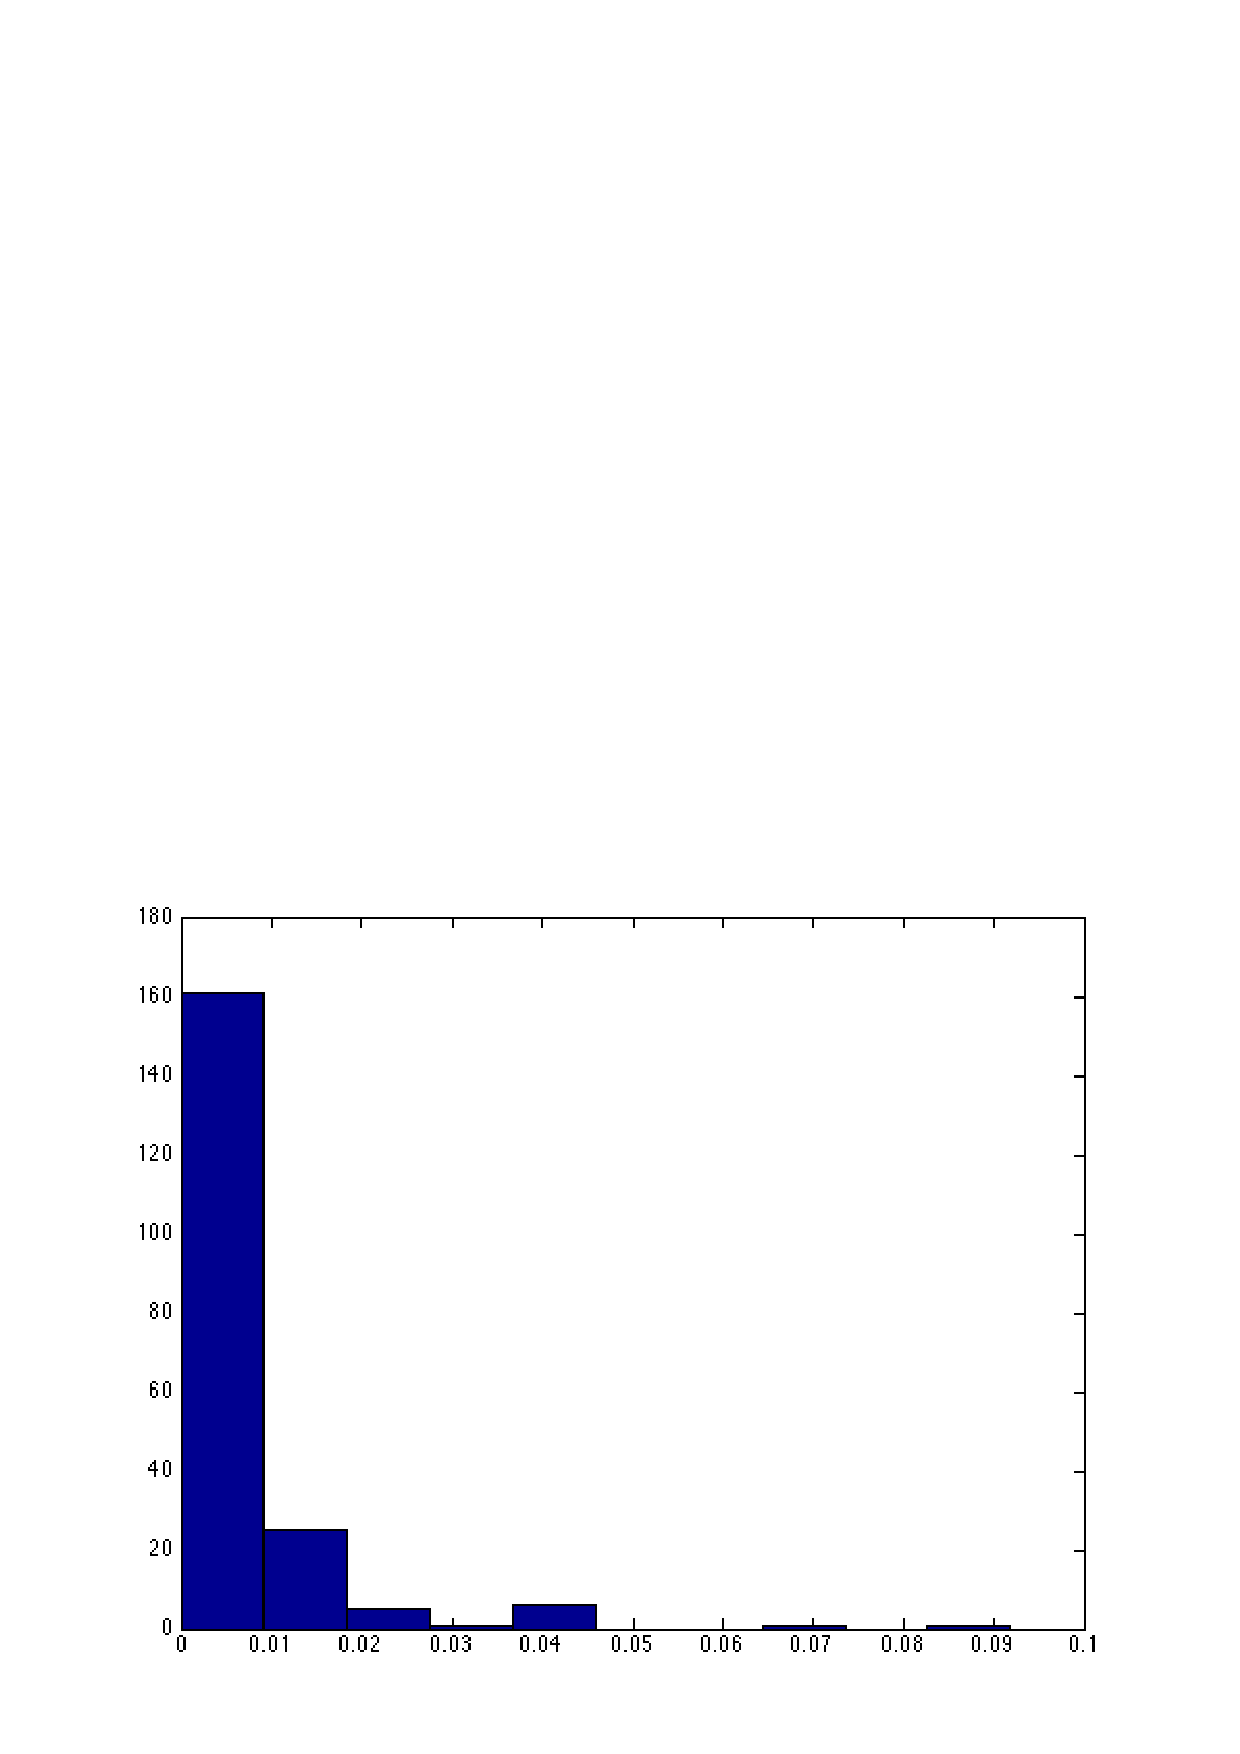
\includegraphics[width=0.45\linewidth]{./Figure/Train_features.png}
    (b)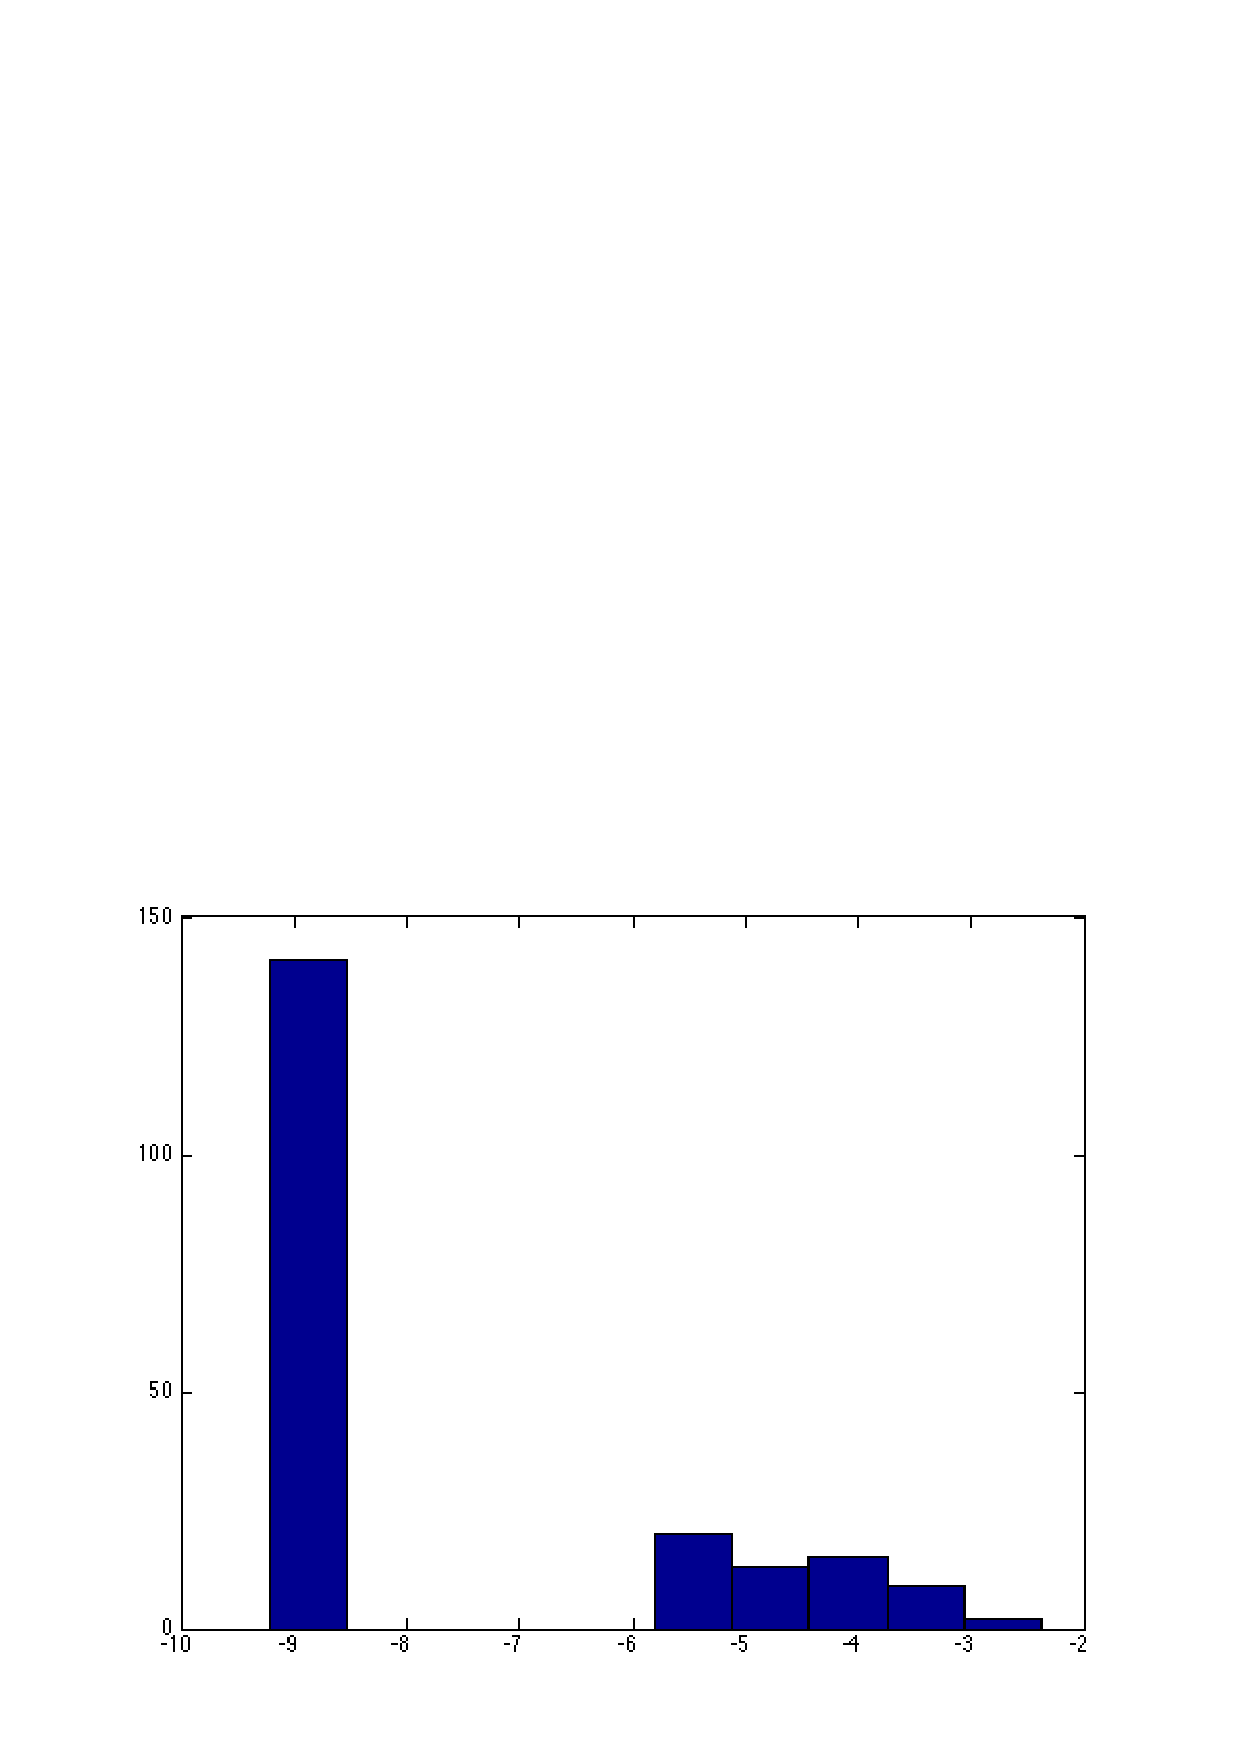
\includegraphics[width=0.45\linewidth]{./Figure/Train_features_log.png}}
    \caption{(a) is the histogram of second feature. Most of the values are close to zero. (b) is the histogram of the log value of the original data.}
    \label{fig:hist}
\end{figure}


We compare the results using nearest neighbor, support vector machine, random forest and naive bayes classifier.


\begin{center}
\begin{small}
\captionof{table}{\small Accuracy of different classifier}
\begin{tabular}{|c|c|c|c|c|c|}
\hline
    KNN & distance      &accuracy   &SVM    & kernel type       &accuracy\\
\hline
        & chi-square    &62.27      &       &chi-square kernel  &72.73\\
\hline
        & euclidean     &54.09      &       & RBF               &70\\
\hline
RandomForest &         & 7.27           &       & linear            &67.7273\\
\hline
Naive Bayes  & kernel densoty  & 15.91           &       & polynomial        &69.0909\\
\hline
        &               &           &       & Sigmoid           &70.9091\\
\hline
\end{tabular}
\end{small}
\end{center}

We can see from our results that kernel SVM has better performance than the other method. First we show the parameter selection in using RBF kernel. Figure \ref{fig:RBF} shows the accuracy to the penalty term $C$ and the parameter $\gamma$. The parameter we selected are $\gamma = 15$ and $C = 4000$.

\begin{figure}[ht!]
    \centering
    {(a)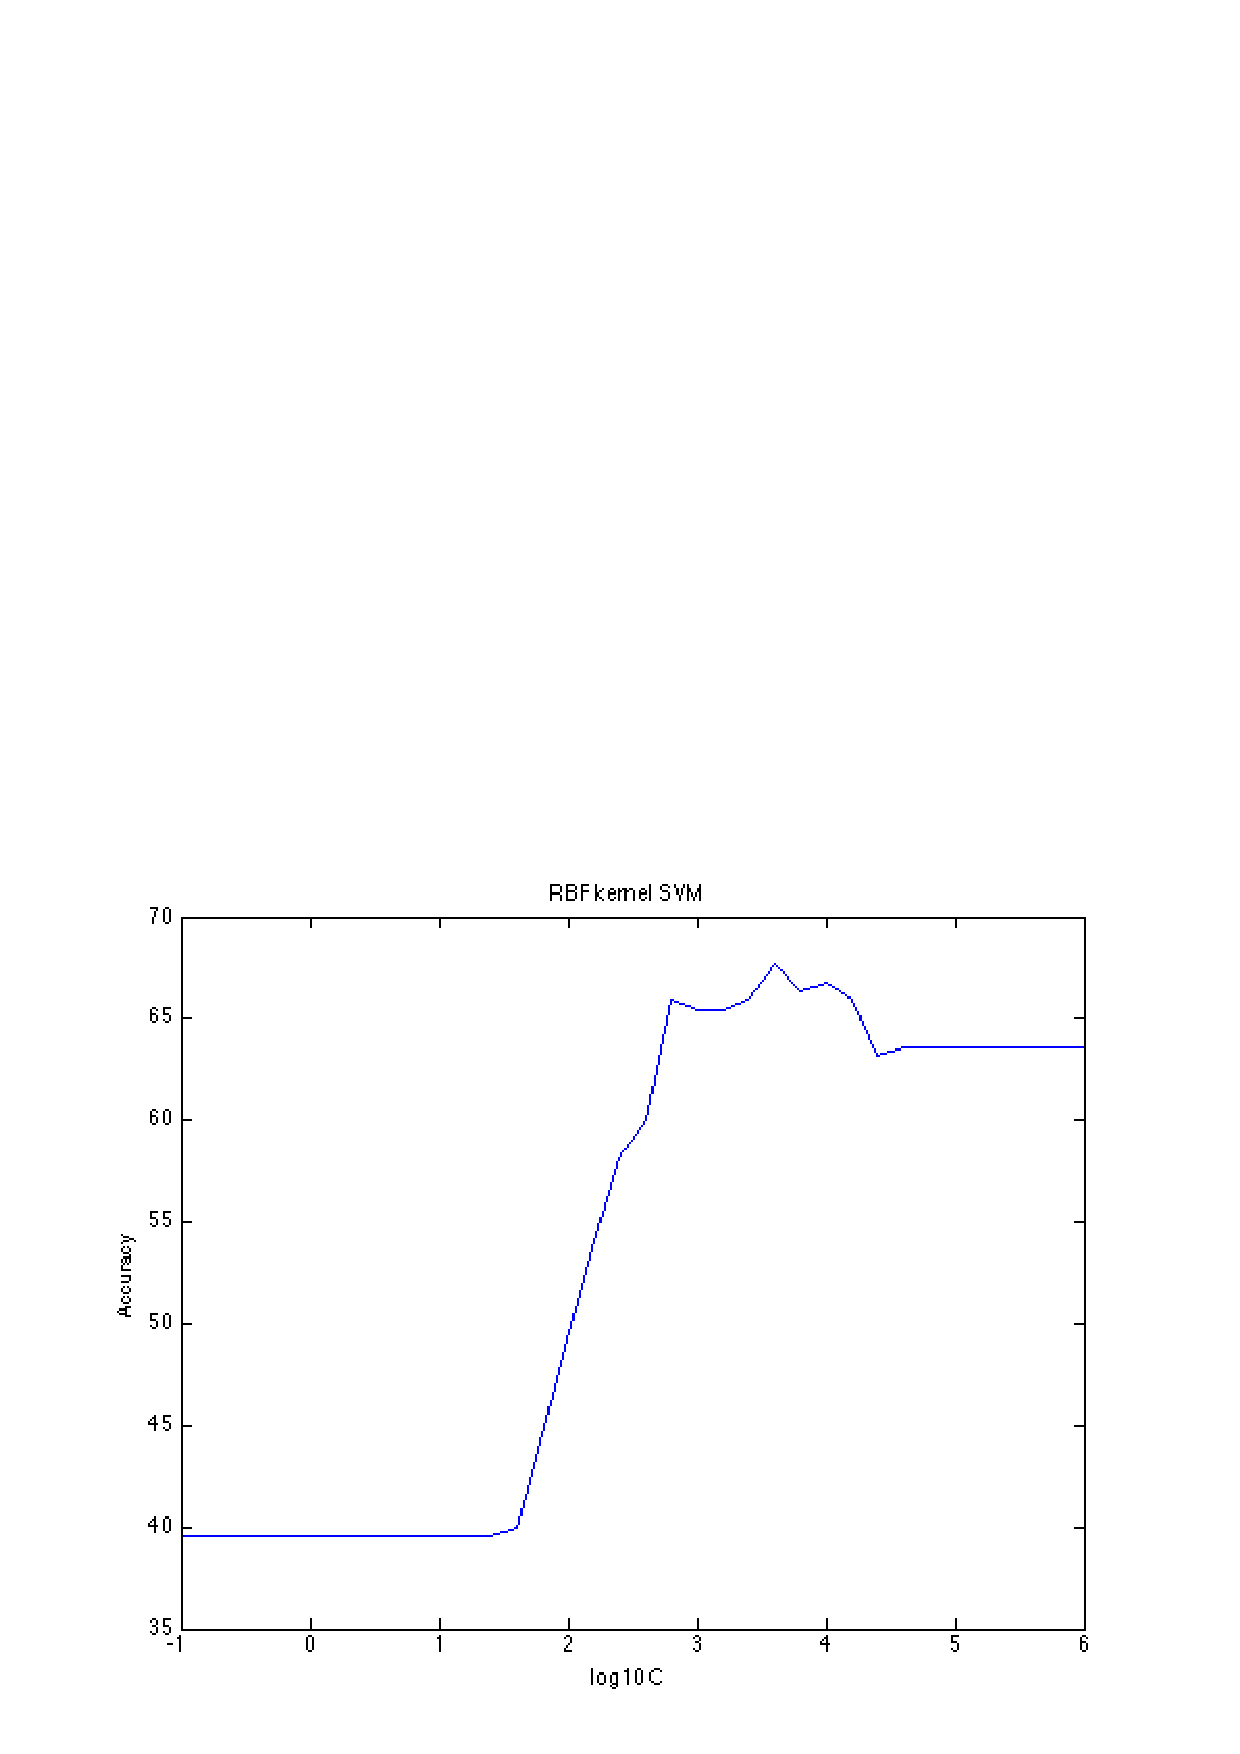
\includegraphics[width=0.45\linewidth]{./Figure/RBF_cost_accuracy.png}
    (b)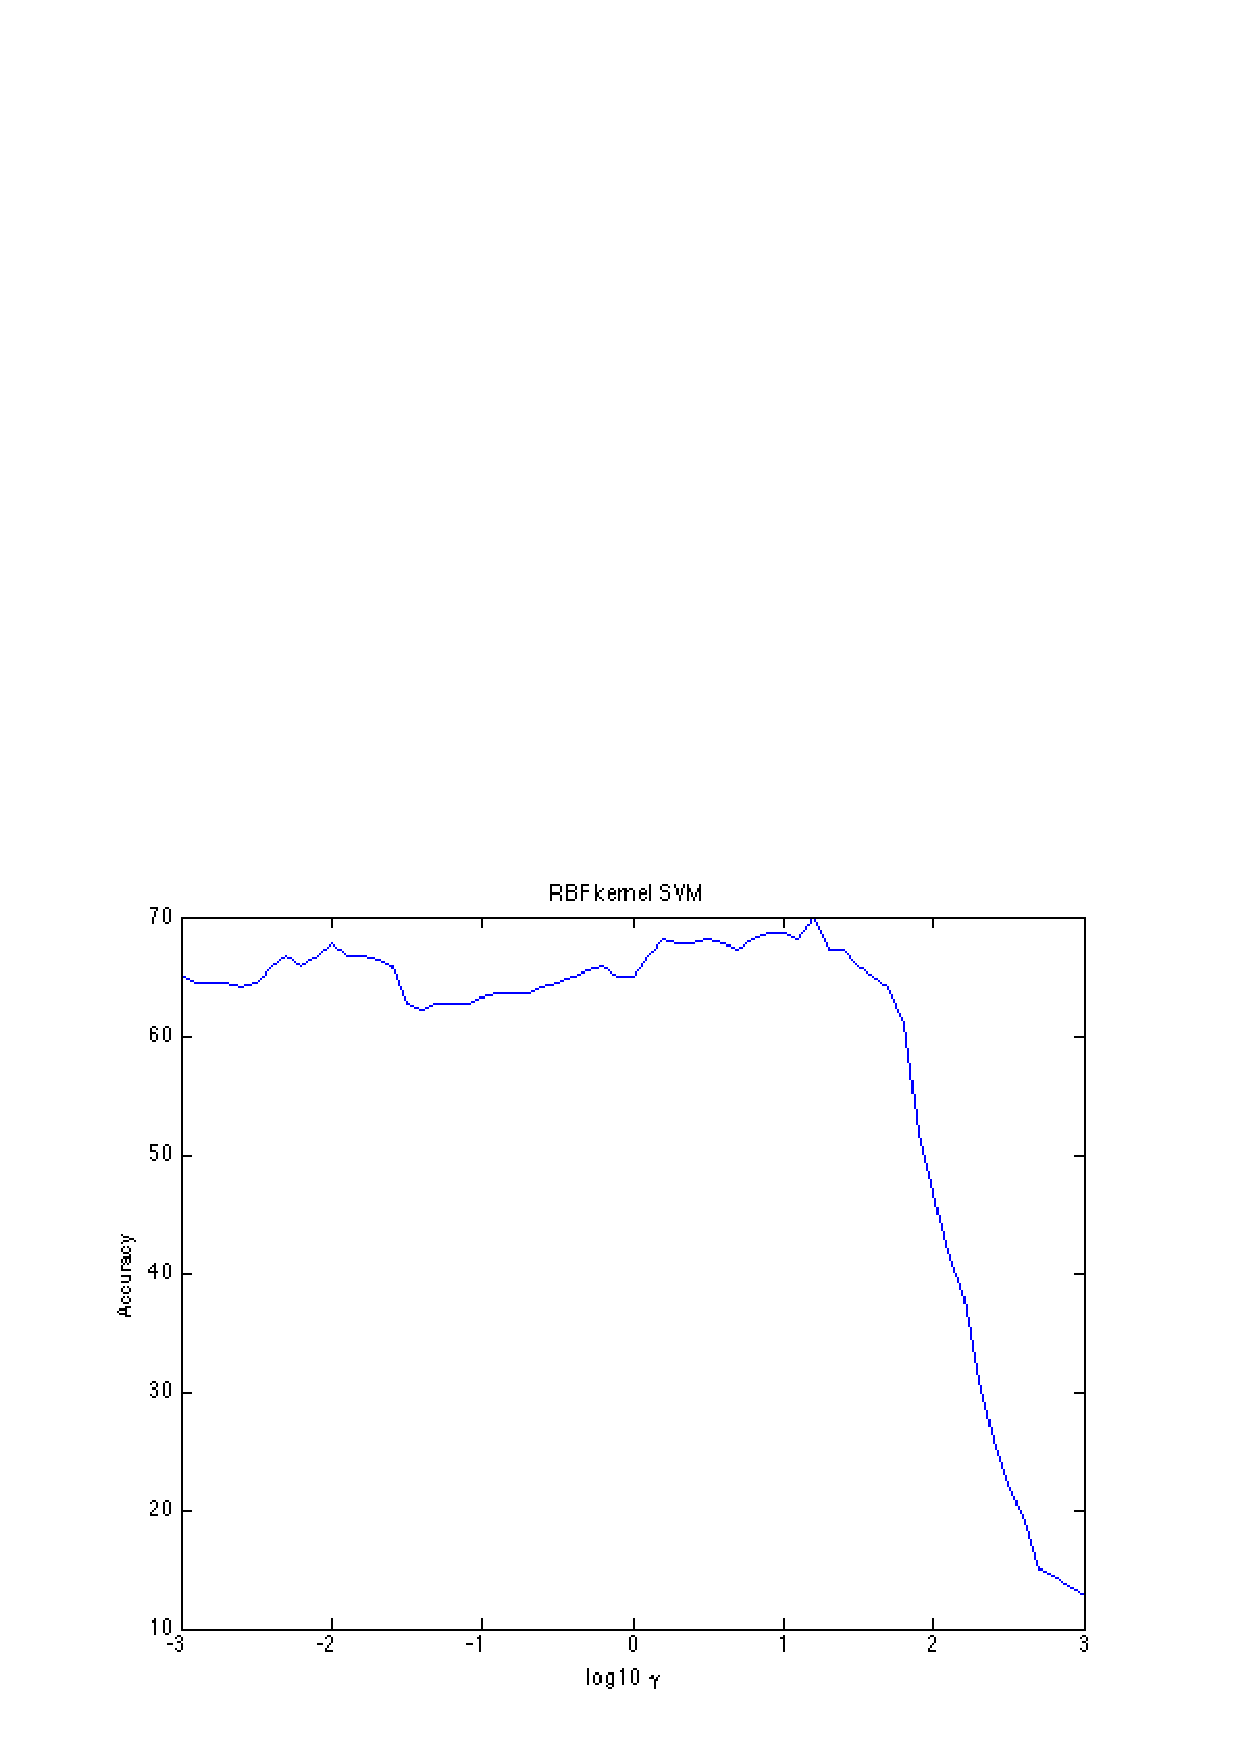
\includegraphics[width=0.45\linewidth]{./Figure/RBF_gamma_accuracy.png}}
    \caption{(a) Accuracy to penalty term c. (b) Accuracy to parameter $\gamma$. }
    \label{fig:RBF}
\end{figure}

In considering that original feature distribution is not a Gaussian distribution, for $x_i,j$ representing the $j^{th}$ feature in the object $i$, we first use a log transformation such that $x_{i,j} = log(x_{i,j} + 0.0001)$ to make the feature distribution more like a combination of Gaussian distribution (see \ref{fig:hist}(b)). The operation leads to a 1.27 improvement in the accuracy after parameter selection process.


\begin{figure}[ht!]
    \centering
    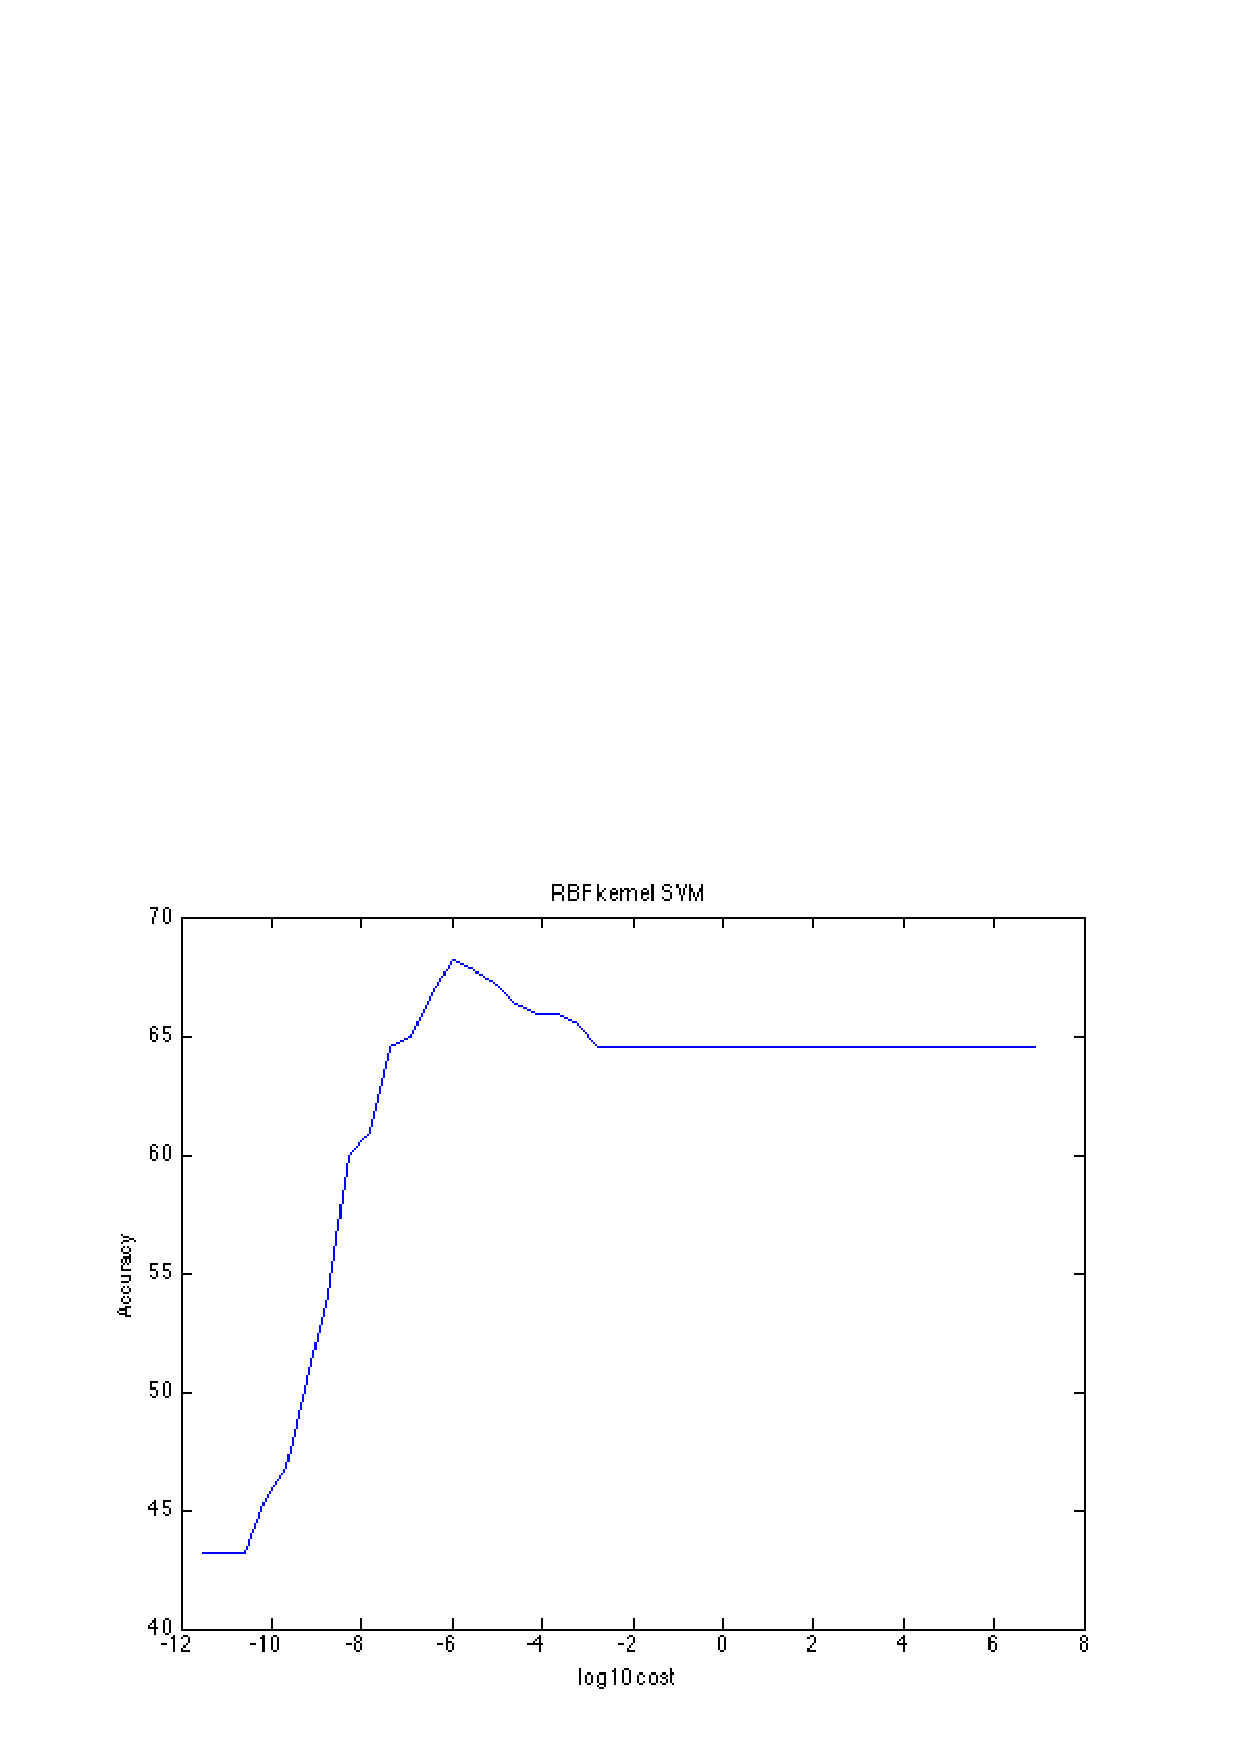
\includegraphics[width=0.45\linewidth]{./Figure/RBF_cost_accuracy_log.png}
     \centering
    \caption{(a) accuracy to penalty C after log transformation on the original feature.}
\end{figure}

Next, we show the results for applying SVM with polynomial kernel. Figure \ref{fig:poly} shows that the performance of accuracy to penalty C is similar to RBF kernel and the optimal value of this parameter is 16000. Besides, according to the experiment results, the optimal degree for the data is around 2. The reason might due to small data size that we use recently so that increasing model complexity will lead to overfitting problem. So we focus on simple model for recent data.  
 
\begin{figure}[ht!]
    \centering
    {(a)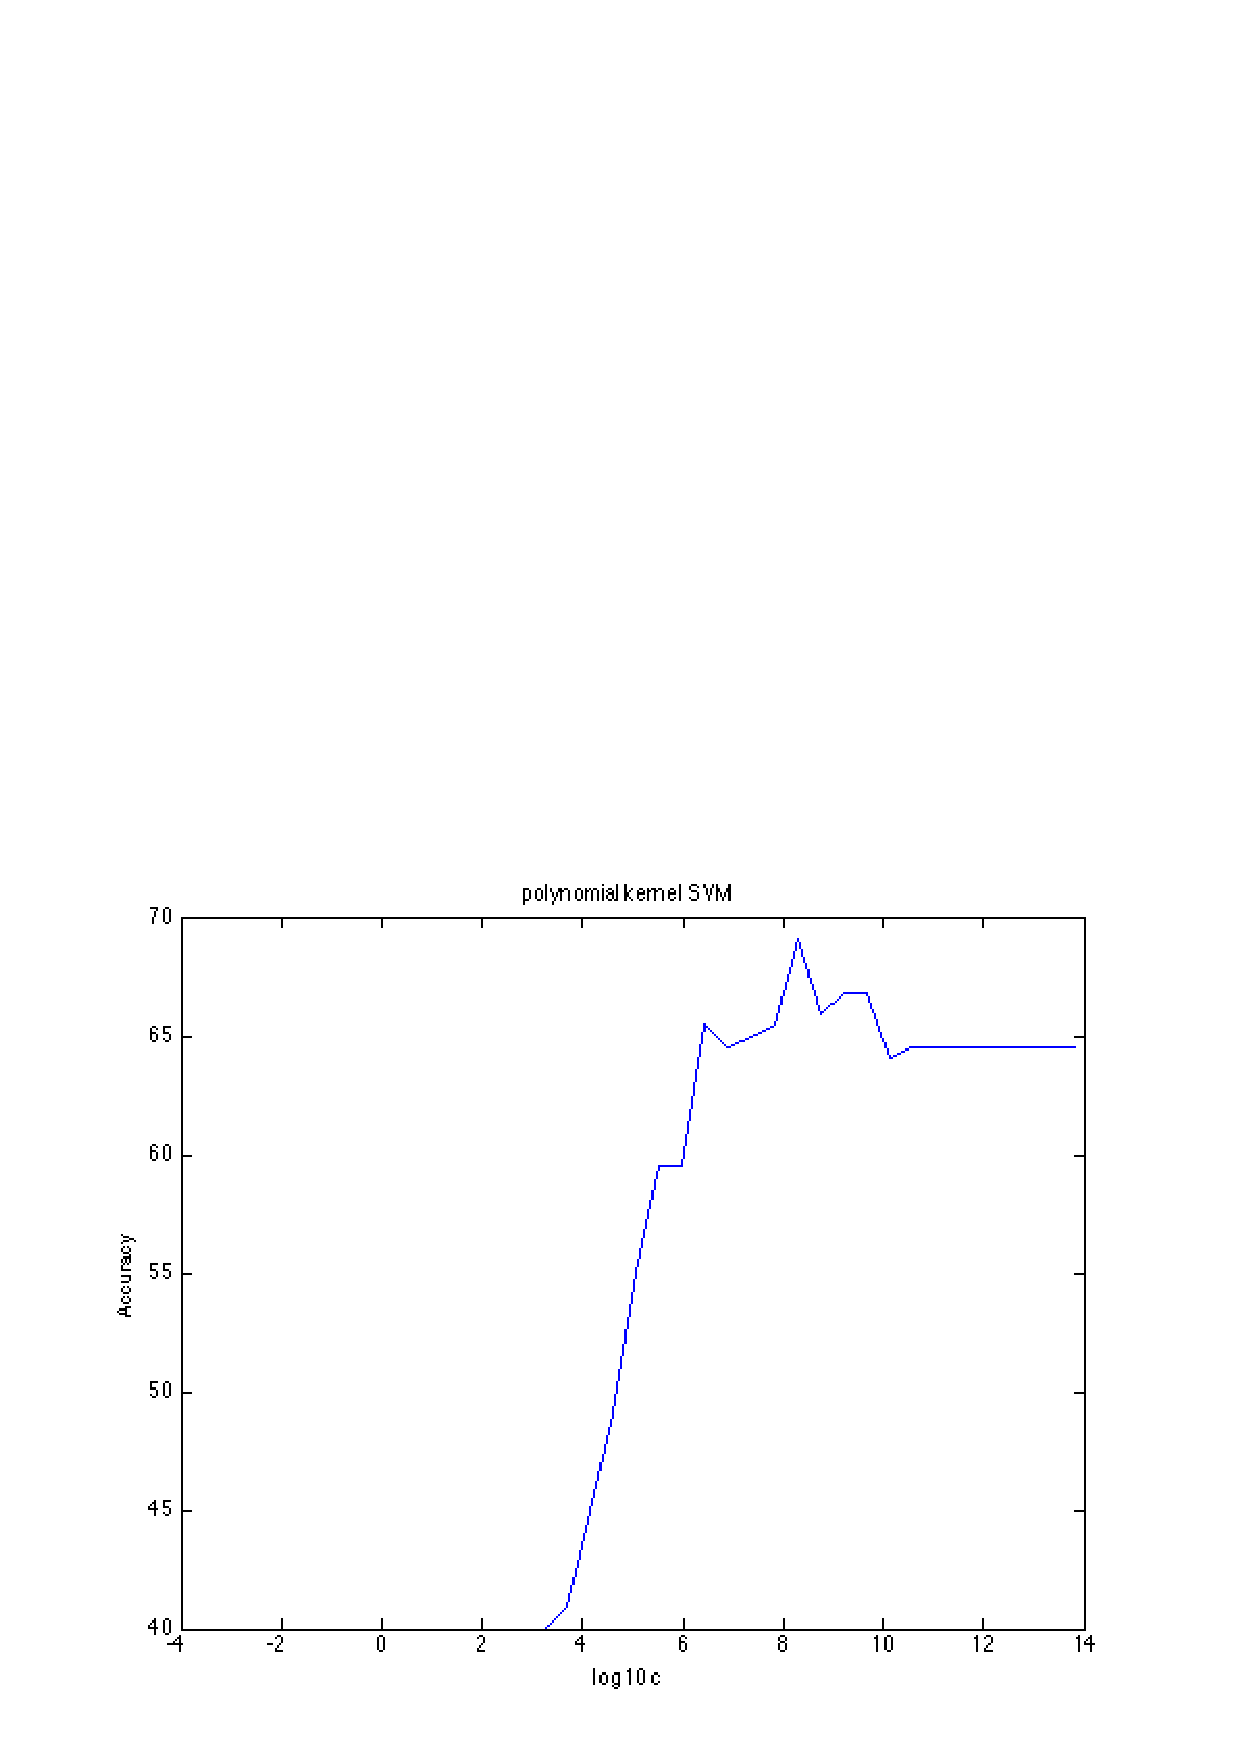
\includegraphics[width=0.45\linewidth]{./Figure/Poly_cost_accuracy.png}
    (b)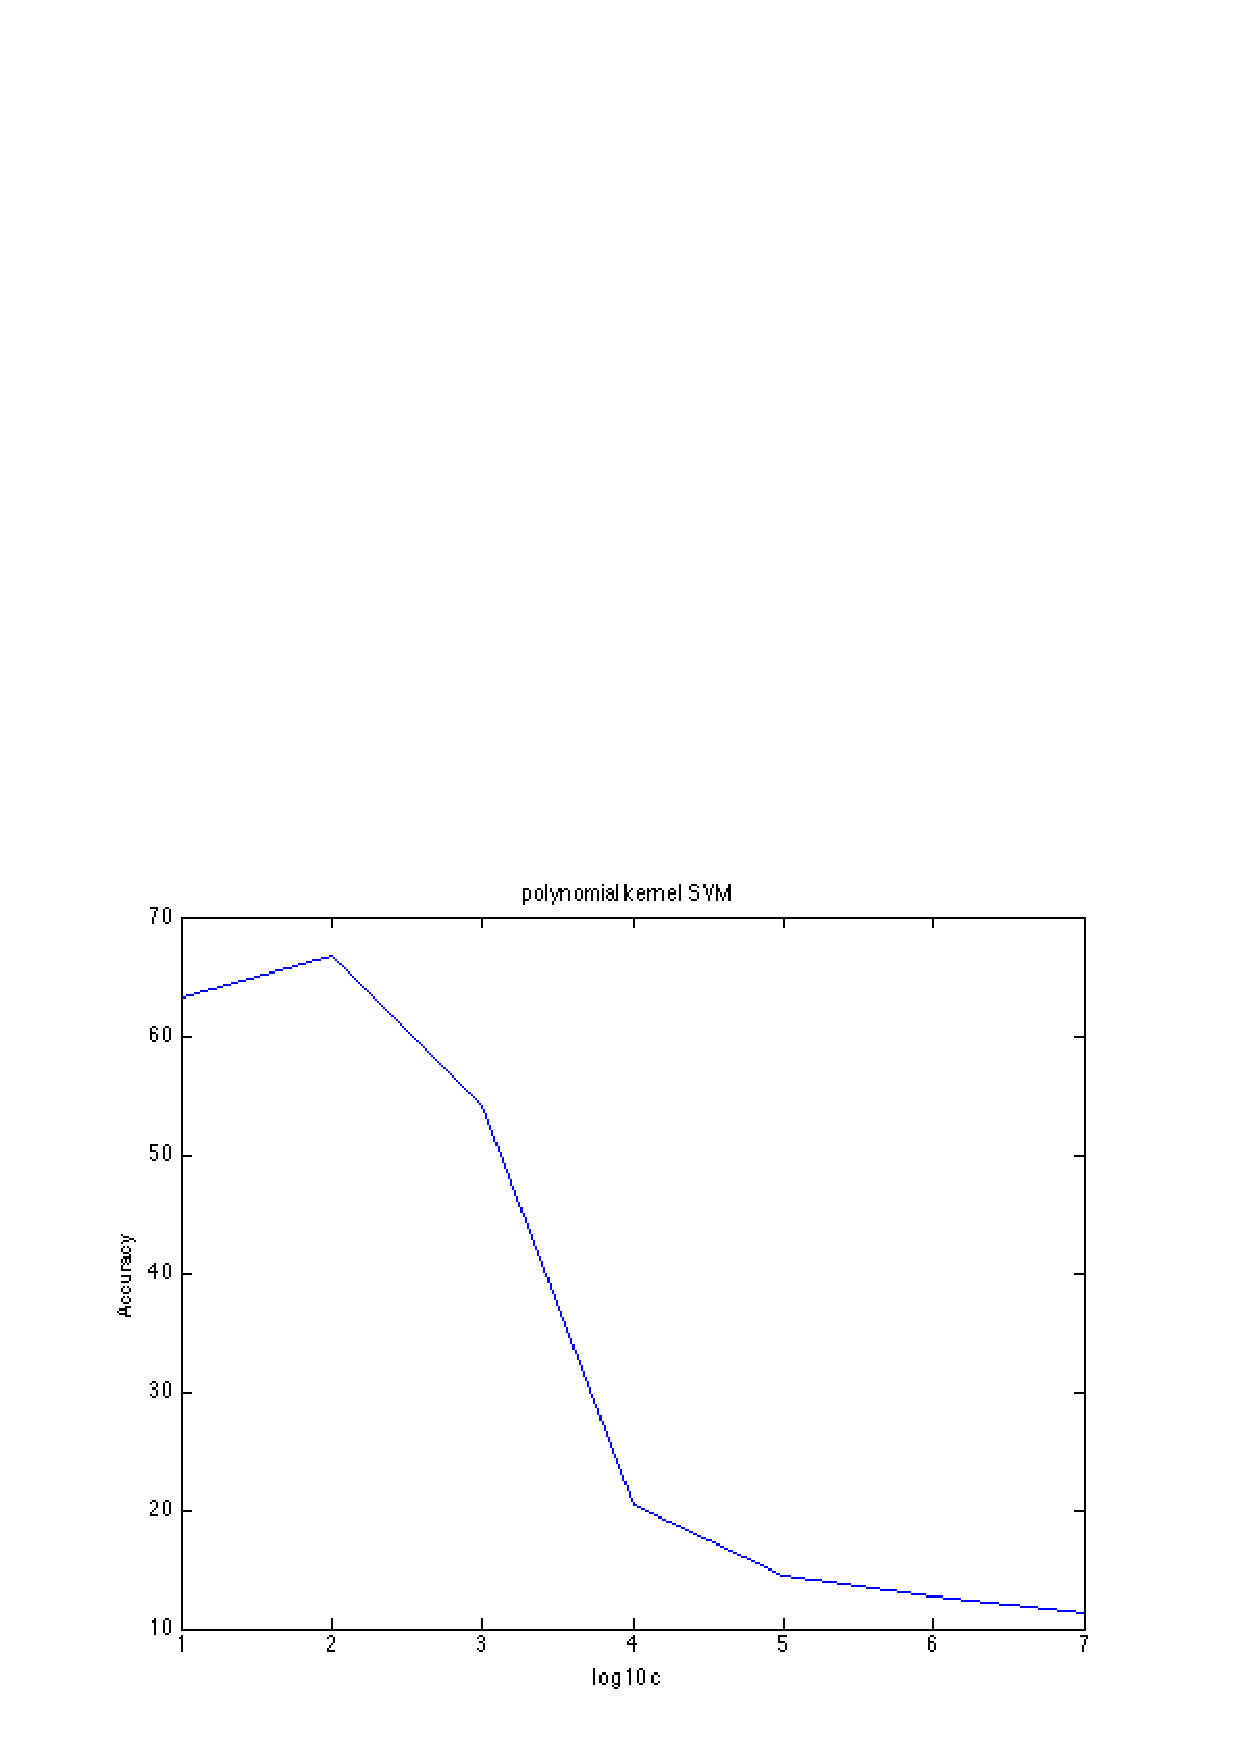
\includegraphics[width=0.45\linewidth]{./Figure/Poly_degree_accuracy.png}}
    \caption{(a) Accuracy to penalty term c. (b) Accuracy to parameter degree d}
    \label{fig:poly}
\end{figure}

The reason why random forest and naive bayes failed is that the training example for each species is now limited to 80. From the predicted classification labels from the results of random forest, we found that the identities in some of the class are all misclassfied into another class, which means that the tree is ill-trained and biased such that many cases will be made to the same decision. 


\bibliographystyle{abbrv}
\bibliography{birds}

\end{document}
